\documentclass[border=0pt]{standalone}
\usepackage[T1]{fontenc}
\usepackage[tt=false,type1=true]{libertine}
\usepackage{tikz}
\pdfinfoomitdate=1
\pdftrailerid{}
\pdfsuppressptexinfo=15
\definecolor{ink}{HTML}{111111}
\definecolor{muted}{HTML}{555555}
\definecolor{grid}{HTML}{808080}
\definecolor{band}{HTML}{F5F5F5}
\definecolor{white}{HTML}{FFFFFF}
\definecolor{m0}{HTML}{DE8F05}
\definecolor{t0}{HTML}{A66700}
\definecolor{m1}{HTML}{0173B2}
\definecolor{t1}{HTML}{0173B2}
\definecolor{m2}{HTML}{029E73}
\definecolor{t2}{HTML}{00855F}
\definecolor{m3}{HTML}{CC78BC}
\definecolor{t3}{HTML}{A45C96}
\definecolor{m4}{HTML}{D55E00}
\definecolor{t4}{HTML}{C35300}
\begin{document}
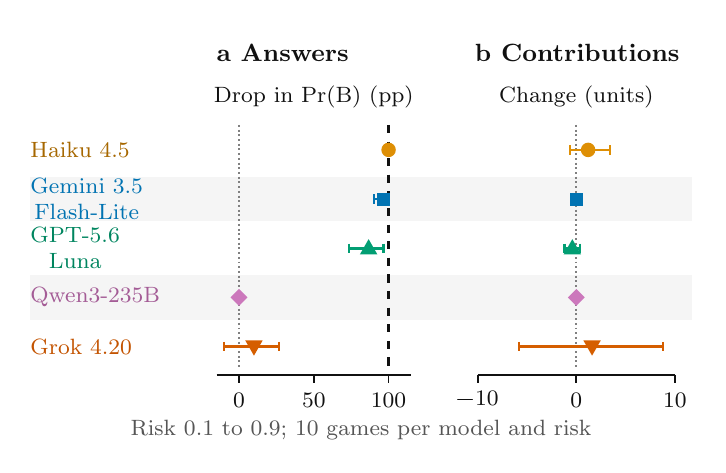
\begin{tikzpicture}[x=1bp,y=-1bp,text=ink,every node/.style={inner sep=0pt,outer sep=0pt,font=\fontsize{8.25}{9.5}\selectfont}]
\path[use as bounding box] (0,0) rectangle (241.1475,150.0);
\fill[band] (1.00000,53.70000) rectangle (239.00000,69.70000);
\fill[band] (1.00000,89.10000) rectangle (239.00000,105.10000);
\node[anchor=west,align=center,text=ink,font=\fontsize{9.2}{10}\selectfont\bfseries] at (68.00000,9.00000) {a  Answers};
\node[anchor=west,align=center,text=ink,font=\fontsize{9.2}{10}\selectfont\bfseries] at (161.00000,9.00000) {b  Contributions};
\node[anchor=center,align=center,text=ink] at (103.00000,25.00000) {Drop in Pr(B) (pp)};
\node[anchor=center,align=center,text=ink] at (197.50000,25.00000) {Change (units)};
\draw[draw=grid,line width=0.7bp,opacity=1,densely dotted] (76.07692,35.00000) -- (76.07692,123.00000);
\draw[draw=grid,line width=0.7bp,opacity=1,densely dotted] (197.50000,35.00000) -- (197.50000,123.00000);
\draw[draw=ink,line width=0.8bp,opacity=1,dashed] (129.92308,35.00000) -- (129.92308,123.00000);
\node[anchor=west,align=center,text=t0] at (1.00000,44.00000) {Haiku 4.5};
\draw[draw=m0,line width=1.0bp,opacity=1] (129.92308,44.00000) -- (129.92308,44.00000);
\draw[draw=m0,line width=0.8bp,opacity=1] (129.92308,42.30000) -- (129.92308,45.70000);
\draw[draw=m0,line width=0.8bp,opacity=1] (129.92308,42.30000) -- (129.92308,45.70000);
\path[draw=m0,fill=m0,line width=0.8bp] (129.92308,44.00000) circle[radius=2.2bp];
\draw[draw=m0,line width=1.0bp,opacity=1] (195.37000,44.00000) -- (209.57000,44.00000);
\draw[draw=m0,line width=0.8bp,opacity=1] (195.37000,42.30000) -- (195.37000,45.70000);
\draw[draw=m0,line width=0.8bp,opacity=1] (209.57000,42.30000) -- (209.57000,45.70000);
\path[draw=m0,fill=m0,line width=0.8bp] (201.76000,44.00000) circle[radius=2.2bp];
\node[anchor=west,align=center,text=t1] at (1.00000,61.70000) {Gemini 3.5\\Flash-Lite};
\draw[draw=m1,line width=1.0bp,opacity=1] (124.53846,61.70000) -- (129.92308,61.70000);
\draw[draw=m1,line width=0.8bp,opacity=1] (124.53846,60.00000) -- (124.53846,63.40000);
\draw[draw=m1,line width=0.8bp,opacity=1] (129.92308,60.00000) -- (129.92308,63.40000);
\path[draw=m1,fill=m1,line width=0.8bp] (126.17021,59.74200) rectangle (130.08621,63.65800);
\draw[draw=m1,line width=1.0bp,opacity=1] (197.50000,61.70000) -- (197.50000,61.70000);
\draw[draw=m1,line width=0.8bp,opacity=1] (197.50000,60.00000) -- (197.50000,63.40000);
\draw[draw=m1,line width=0.8bp,opacity=1] (197.50000,60.00000) -- (197.50000,63.40000);
\path[draw=m1,fill=m1,line width=0.8bp] (195.54200,59.74200) rectangle (199.45800,63.65800);
\node[anchor=west,align=center,text=t2] at (1.00000,79.40000) {GPT-5.6\\Luna};
\draw[draw=m2,line width=1.0bp,opacity=1] (115.56410,79.40000) -- (128.12821,79.40000);
\draw[draw=m2,line width=0.8bp,opacity=1] (115.56410,77.70000) -- (115.56410,81.10000);
\draw[draw=m2,line width=0.8bp,opacity=1] (128.12821,77.70000) -- (128.12821,81.10000);
\path[draw=m2,fill=m2,line width=0.8bp] (122.74359,76.93600) -- (125.20759,81.24800) -- (120.27959,81.24800) -- cycle;
\draw[draw=m2,line width=1.0bp,opacity=1] (193.24000,79.40000) -- (198.92000,79.40000);
\draw[draw=m2,line width=0.8bp,opacity=1] (193.24000,77.70000) -- (193.24000,81.10000);
\draw[draw=m2,line width=0.8bp,opacity=1] (198.92000,77.70000) -- (198.92000,81.10000);
\path[draw=m2,fill=m2,line width=0.8bp] (196.08000,76.93600) -- (198.54400,81.24800) -- (193.61600,81.24800) -- cycle;
\node[anchor=west,align=center,text=t3] at (1.00000,97.10000) {Qwen3-235B};
\draw[draw=m3,line width=1.0bp,opacity=1] (76.07692,97.10000) -- (76.07692,97.10000);
\draw[draw=m3,line width=0.8bp,opacity=1] (76.07692,95.40000) -- (76.07692,98.80000);
\draw[draw=m3,line width=0.8bp,opacity=1] (76.07692,95.40000) -- (76.07692,98.80000);
\path[draw=m3,fill=m3,line width=0.8bp] (76.07692,94.63600) -- (78.54092,97.10000) -- (76.07692,99.56400) -- (73.61292,97.10000) -- cycle;
\draw[draw=m3,line width=1.0bp,opacity=1] (197.50000,97.10000) -- (197.50000,97.10000);
\draw[draw=m3,line width=0.8bp,opacity=1] (197.50000,95.40000) -- (197.50000,98.80000);
\draw[draw=m3,line width=0.8bp,opacity=1] (197.50000,95.40000) -- (197.50000,98.80000);
\path[draw=m3,fill=m3,line width=0.8bp] (197.50000,94.63600) -- (199.96400,97.10000) -- (197.50000,99.56400) -- (195.03600,97.10000) -- cycle;
\node[anchor=west,align=center,text=t4] at (1.00000,114.80000) {Grok 4.20};
\draw[draw=m4,line width=1.0bp,opacity=1] (70.69231,114.80000) -- (90.43590,114.80000);
\draw[draw=m4,line width=0.8bp,opacity=1] (70.69231,113.10000) -- (70.69231,116.50000);
\draw[draw=m4,line width=0.8bp,opacity=1] (90.43590,113.10000) -- (90.43590,116.50000);
\path[draw=m4,fill=m4,line width=0.8bp] (81.46154,117.26400) -- (83.92554,112.95200) -- (78.99754,112.95200) -- cycle;
\draw[draw=m4,line width=1.0bp,opacity=1] (176.91000,114.80000) -- (228.74000,114.80000);
\draw[draw=m4,line width=0.8bp,opacity=1] (176.91000,113.10000) -- (176.91000,116.50000);
\draw[draw=m4,line width=0.8bp,opacity=1] (228.74000,113.10000) -- (228.74000,116.50000);
\path[draw=m4,fill=m4,line width=0.8bp] (203.18000,117.26400) -- (205.64400,112.95200) -- (200.71600,112.95200) -- cycle;
\draw[draw=ink,line width=0.7bp,opacity=1] (68.00000,125.00000) -- (138.00000,125.00000);
\draw[draw=ink,line width=0.7bp,opacity=1] (162.00000,125.00000) -- (233.00000,125.00000);
\draw[draw=ink,line width=0.6bp,opacity=1] (76.07692,125.00000) -- (76.07692,128.00000);
\node[anchor=center,align=center,text=ink] at (76.07692,134.00000) {0};
\draw[draw=ink,line width=0.6bp,opacity=1] (103.00000,125.00000) -- (103.00000,128.00000);
\node[anchor=center,align=center,text=ink] at (103.00000,134.00000) {50};
\draw[draw=ink,line width=0.6bp,opacity=1] (129.92308,125.00000) -- (129.92308,128.00000);
\node[anchor=center,align=center,text=ink] at (129.92308,134.00000) {100};
\draw[draw=ink,line width=0.6bp,opacity=1] (162.00000,125.00000) -- (162.00000,128.00000);
\node[anchor=center,align=center,text=ink] at (162.00000,134.00000) {\textminus10};
\draw[draw=ink,line width=0.6bp,opacity=1] (197.50000,125.00000) -- (197.50000,128.00000);
\node[anchor=center,align=center,text=ink] at (197.50000,134.00000) {0};
\draw[draw=ink,line width=0.6bp,opacity=1] (233.00000,125.00000) -- (233.00000,128.00000);
\node[anchor=center,align=center,text=ink] at (233.00000,134.00000) {10};
\node[anchor=center,align=center,text=muted] at (120.00000,145.00000) {Risk 0.1 to 0.9; 10 games per model and risk};
\end{tikzpicture}
\end{document}
